\documentclass[aspectratio=169, 12pt]{beamer}
\usepackage{bbm}
\usepackage[utf8]{inputenc}
\usepackage[T2A]{fontenc}
\usepackage[english]{babel}
\usepackage{amscd,amssymb}
\usepackage{amsfonts,amsmath,array}
\usepackage{sidecap}
\usepackage[T2A]{fontenc}
\usepackage[utf8]{inputenc}
\usepackage{graphicx}				% Вставка картинок правильная
\DeclareGraphicsExtensions{.pdf,.png,.jpg}
\usepackage{pdfpages}
\usepackage{multicol}

% Для алгоритмов
\usepackage{amsmath}
\usepackage{amsthm}
\usepackage{amssymb}
\usepackage{mathtools}
\usepackage{algorithm}
\usepackage{algpseudocode}
% Цвета
\usepackage{color}
\usepackage{colortbl}
% Создаем новую команду для assumptions
%----------------------------------------------------------------------------------------------------------

\newtheorem{assumption}{Assumption}
%beamer  theme's used to be here :)
%\usetheme{mipt_beamer}
\usetheme{boxes}

%----------------------------------------------------------------------------------------------------------
\title[\hbox to 56mm{Feature}]{Neural Networks Fail to Learn Periodic Functions and How to Fix It}
\author[V.\,M.~Minashkin]{Vladislav Minashkin, MSc.}
\institute{Moscow Institute of Physics and Technology}
\date{\today}

\begin{document}
\maketitle

\begin{frame}{Table of contents}
    \tableofcontents
\end{frame}

% Slide for task/model motivation
\section{Task/Model Motivation}
\begin{frame}
\frametitle{Task/Model Motivation}
\begin{itemize}
    \item Periodic functions are crucial in modeling natural and societal phenomena (e.g., biological clocks, economic cycles).
    \item Standard neural networks (e.g., with ReLU, tanh) struggle to extrapolate periodic functions beyond training data.
    \item Need for a flexible model that handles both periodic and non-periodic functions without prior knowledge of periodicity.
\end{itemize}
\end{frame}

\begin{frame}

       \begin{center}
       \begin{figure}
           \centering
           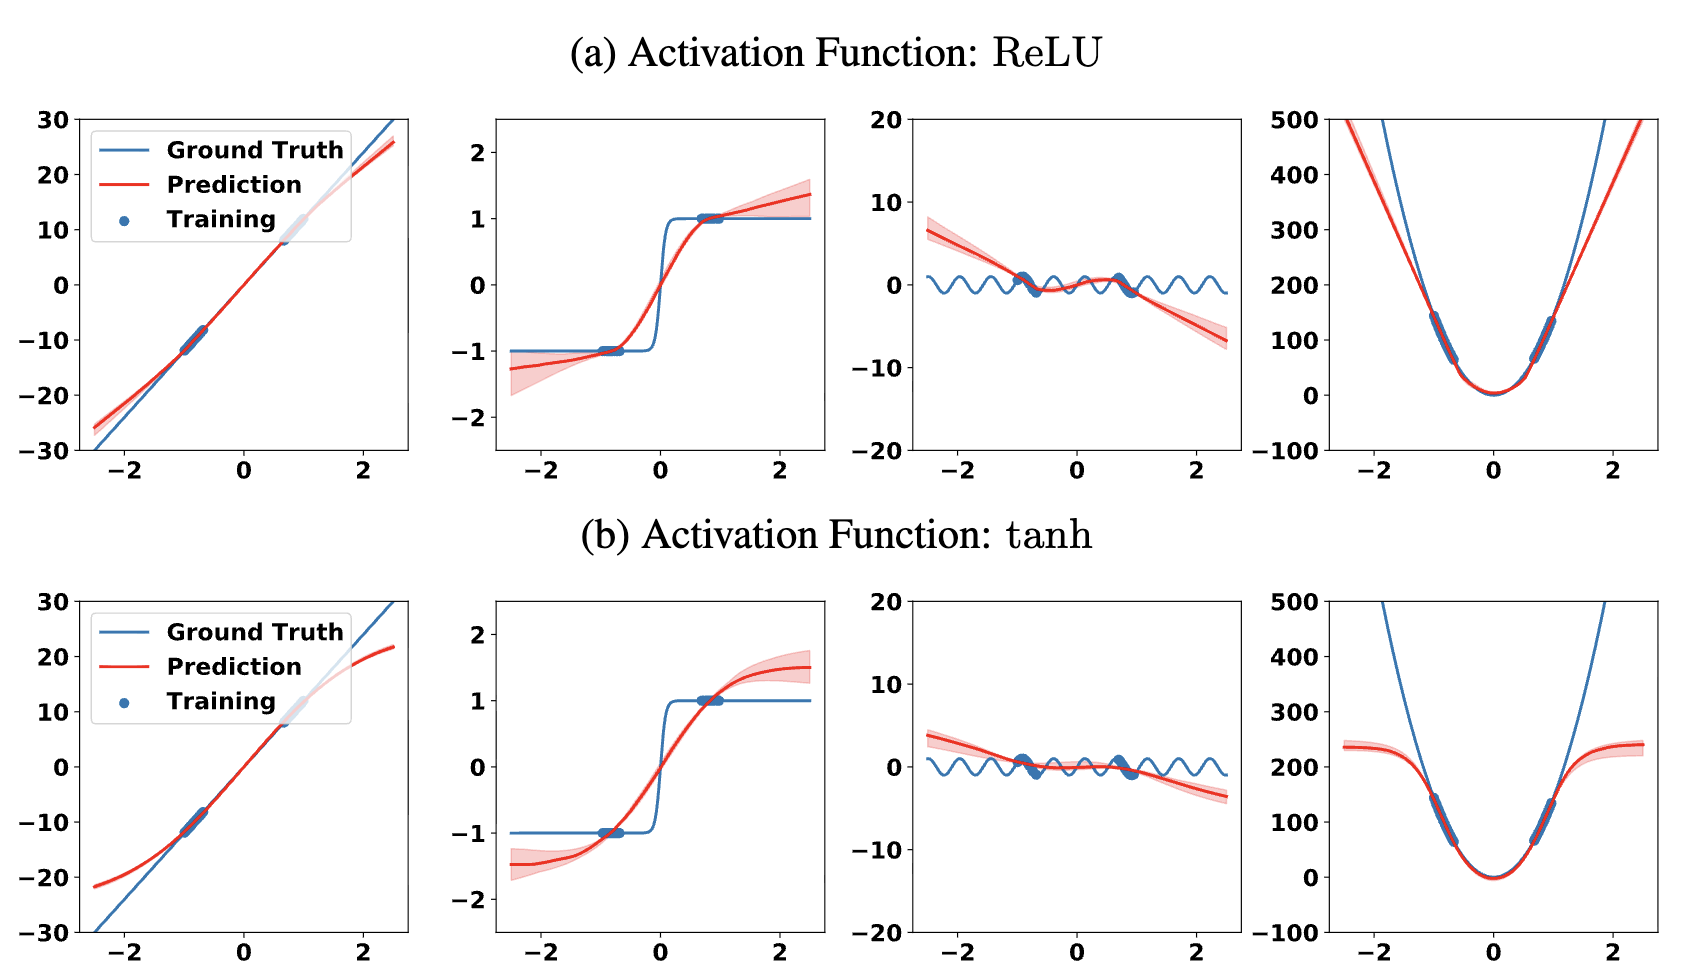
\includegraphics[width=0.6\textwidth]{1.png}
           \caption{Exploration of how different activation functions extrapolate various basic function types: $y = x$ (first column), $y = \tanh(x)$ (second column), $y = \sin(x)$ (third column), and $y = x^2$ (last column). The red curves represents the median model prediction and the shaded regions show the 90\% credibility interval from 21 independent runs. Note that the horizontal range is re-scaled so that the training data lies between -1 and 1.
}
       \end{figure}

        \end{center}
\end{frame}

% Slide for formal problem statement
\section{Formal Problem Statement}
\begin{frame}
\frametitle{Formal Problem Statement}
\begin{definition}[Feedforward Neural Network]
Let $f_{\sigma}(x) = W_{h} \sigma \ldots \sigma W_{1} x$ be a function from $\mathbb{R}^{d_{1}} \rightarrow \mathbb{R}^{d_{h+1}}$, where $\sigma$ is the activation function applied element-wise to its input vector, and $W_{i} \in \mathbb{R}^{d_{i} \times d_{i+1}}$. $f_{\sigma}(x)$ is called a feedforward neural network with activation function $\sigma$, and $d_{1}$ is called the input dimension, and $d_{h+1}$ is the output dimension.
\end{definition}
\end{frame}

\begin{frame}
\frametitle{Formal Problem Statement}
\begin{theorem}[ReLU Extrapolation]
Consider a feed forward network $f_{\text{ReLU}}(x)$, with arbitrary but fixed depth $h$ and widths $d_{1}, \ldots, d_{h+1}$. Then

$$ \lim_{z \to \infty} \| f_{\text{ReLU}}(zu) - z W_{u} u - b_{u} \| = 0, $$

where $z$ is a real scalar, $u$ is any unit vector of dimension $d_{1}$, and $W_{u} \in \mathbb{R}^{d_{1} \times d_{h}}$ is a constant matrix only dependent on $u$.
\end{theorem}
\end{frame}


\begin{frame}
\frametitle{Formal Problem Statement}
\begin{theorem}[Tanh Extrapolation]
Consider a feed forward network $f_{\text{tanh}}(x)$, with arbitrarily fixed depth $h$ and widths $d_{1}, \ldots, d_{h+1}$. Then

$$ \lim_{z \to \infty} \| f_{\text{tanh}}(zu) - v_{u} \| = 0, $$

where $z$ is a real scalar, $u$ is any unit vector of dimension $d_{1}$, and $v_{u} \in \mathbb{R}^{d_{h+1}}$ is a constant vector that only depends on $u$.
\end{theorem}
\end{frame}

% Slide for theory and method description
\section{Theory and Method Description}
\begin{frame}
\frametitle{Theory and Method Description}
\begin{itemize}
    \item \textbf{Theory}: Standard activations (ReLU, tanh) extrapolate linearly or to constants, unsuitable for periodic functions (Theorems 1 and 2).
    \item \textbf{Proposed Method}: Introduce \textit{Snake} activation function: \( \text{Snake}_a(x) = x + \frac{1}{a} \sin^2(ax) \).
    \item \textbf{Advantages}: Periodic inductive bias, monotonicity, and second-order non-linear term for better approximation.
    \item \textbf{Initialization}: Adjusted for unit variance, with learnable frequency parameter \( a \).
\end{itemize}
\end{frame}

\begin{frame}
\frametitle{Theory and Method Description}
\begin{theorem}[Snake Universal Extrapolation]
    Let $f(x)$ be a piecewise $C^{1}$ periodic function with period $L$. Then, a Snake neural network, $f_{w_{N}}$, with one hidden layer and with width $N$ can converge to $f(x)$ uniformly as $N \rightarrow \infty$, i.e., there exists parameters $w_{N}$ for all $N \in \mathbb{Z}^{+}$ such that

    $$ f(x) = \lim_{N \rightarrow \infty} f_{w_{N}}(x) $$

    for all $x \in \mathbb{R}$, i.e., the convergence is point-wise. If $f(x)$ is continuous, then the convergence is uniform.
\end{theorem}
\end{frame}

\begin{frame}{Initialization}
     Let $W \in \mathbb{R}^{d_{1} \times d_{2}}$, whose input activations are $h \in \mathbb{R}^{d_{2}}$ with a unit variance for each of its element, and the goal is to set the variance of each element in $W$ such that Snake($Wx$) has a unit variance. To leading order, Snake looks like an identity function, and so one can make this approximation in finding the required variance: $\mathbb{E} \left( \sum_{j}^{d_{2}} W_{ij} x_{j} \right)^{2} = 1$ which gives $\mathbb{E}[W_{ij}^{2}] = 1/d$. If we use uniform distribution to initialize $W$, then we should sample from $Uniform(-\sqrt{\frac{3}{d}}, \sqrt{\frac{3}{d}})$, which is a factor of $\sqrt{2}$ smaller in range than the Kaiming uniform initialization.

 The variance of expected value of $x + \frac{\sin^{2}(ax)}{a}$ under a standard normal distribution is $\sigma_{a}^{2} = 1 + \frac{1 + e^{-8a^{2}} - 2e^{-4a^{2}}}{8a^{2}}$, which is maximized at $a_{max} \approx 0.56045$.

\end{frame}

% Slide for experiments, examples, applications
\section{Experiments, Examples, Applications}
\begin{frame}
\frametitle{Experiments, Examples, Applications}
\begin{itemize}
    \item \textbf{Regression}: Snake successfully extrapolates periodic functions (e.g., \(\sin(x)\)) unlike ReLU/tanh
    \item \textbf{Image Classification}: Competitive with ReLU on CIFAR-10 using ResNet-18/101
    \item \textbf{Real-World Applications}:
        \begin{itemize}
            \item Atmospheric temperature prediction (Minamitorishima): Captures weekly cycles
            \item Human body temperature: Models circadian rhythm with limited data
            \item Financial data: Predicts Wilshire 5000 Index, capturing economic cycles
        \end{itemize}
    \item \textbf{RNN Comparison}: Snake outperforms RNNs in time series tasks with less computational cost
\end{itemize}
\end{frame}


\begin{frame}{Minamitorishima}
    \begin{center}
       \begin{figure}
           \centering
           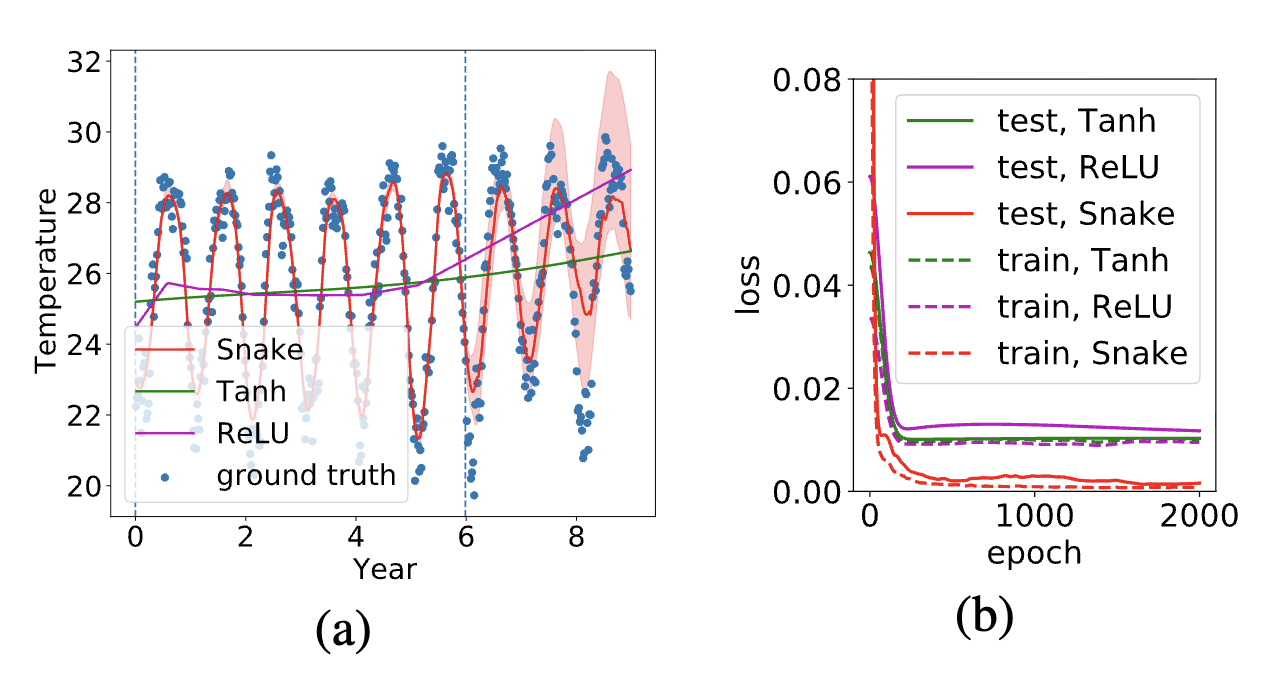
\includegraphics[width=0.6\textwidth]{2.png}
           \caption{Experiment on the atmospheric data. (a) Regressing the mean weekly temperature evolution of Minamitorishima with different activation functions. For Snake, $a$ is treated as a learnable parameter and the red contour shows the 90\% credibility interval. (b) Comparison of tanh, ReLU, and Snake on a regression task with learnable $a$.}
       \end{figure}

        \end{center}
\end{frame}

\begin{frame}{Financial Data}
    \begin{center}
       \begin{figure}
           \centering
           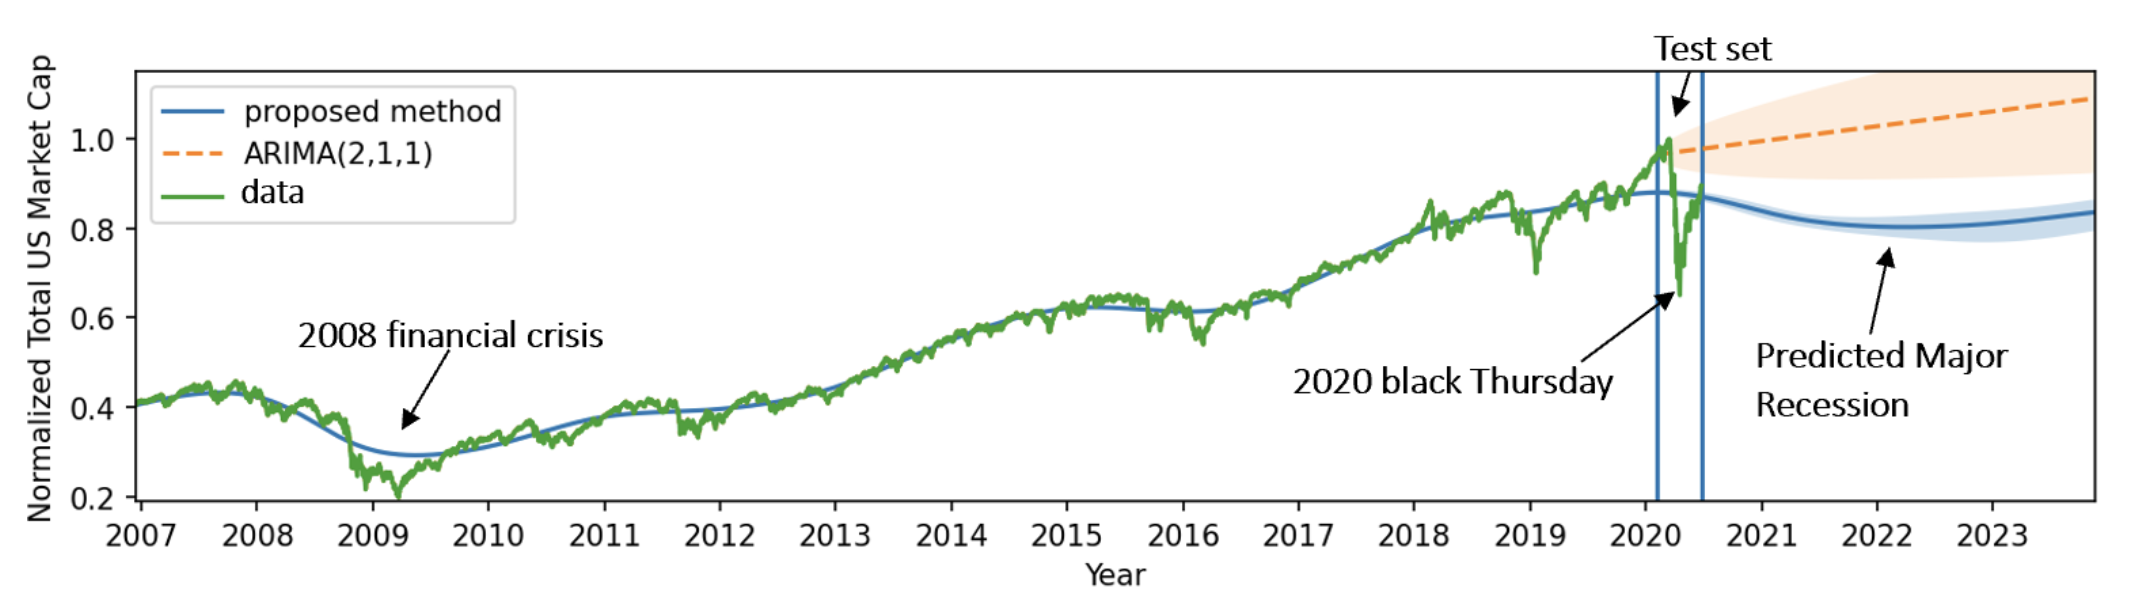
\includegraphics[width=0.8\textwidth]{3.png}
           \caption{Prediction of Wilshire 5000 index, an indicator of the US and global economy.}
       \end{figure}

        \end{center}
\end{frame}

% Slide for literature
\section{Literature}
\begin{frame}
\frametitle{Literature}
\begin{itemize}
    \item Hornik et al. (1989): Universal approximation theorem for neural networks.
    \item He et al. (2015): Kaiming initialization for deep networks.
    \item Ramachandran et al. (2017): Swish activation function.
    \item Parascandolo et al. (2016): Sine as activation function.
    \item Silvescu (1999), Zhumekenov et al. (2019): Fourier neural networks.
    \item Full references in paper: \url{https://proceedings.neurips.cc/paper/2020/file/1160453108d3e537255e9f7b931f4e90-Paper.pdf}
\end{itemize}
\end{frame}

\end{document}
